\chapter{TP3 : Outil de simulation de réseaux : NS-2}
    On commence par réaliser le réseau demandé. Grâce au TP précédent, cela se fait rapidement, et selon les spécifications du sujet.

    En changeant le temps d'enregistrement des courbes nous obtenons un taux d'échantillonage plus ou moins élevé.
    \begin{figure}
      \centering
        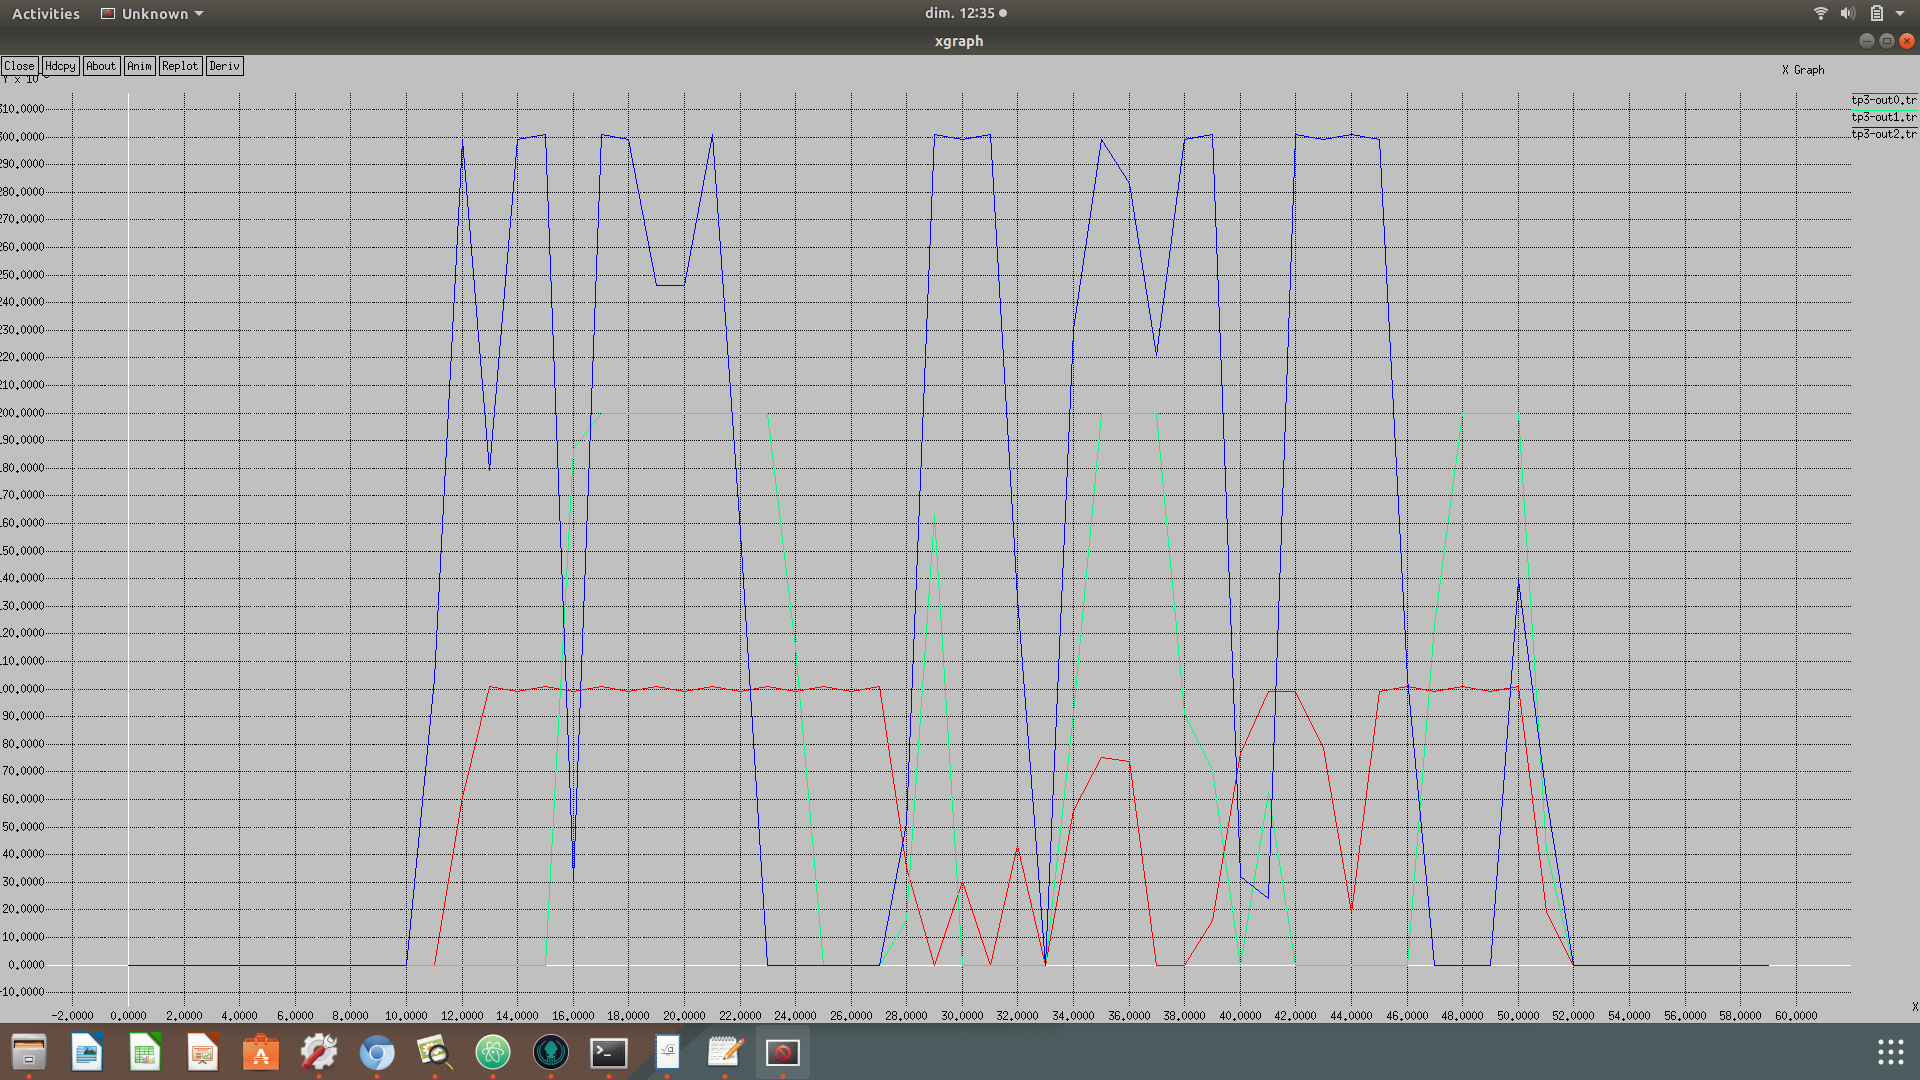
\includegraphics[width=0.99\columnwidth]{./tp3/1,0.png}
        \caption{xGraph : Échantillonage de 1 seconde}
    \end{figure}

    \begin{figure}
      \centering
        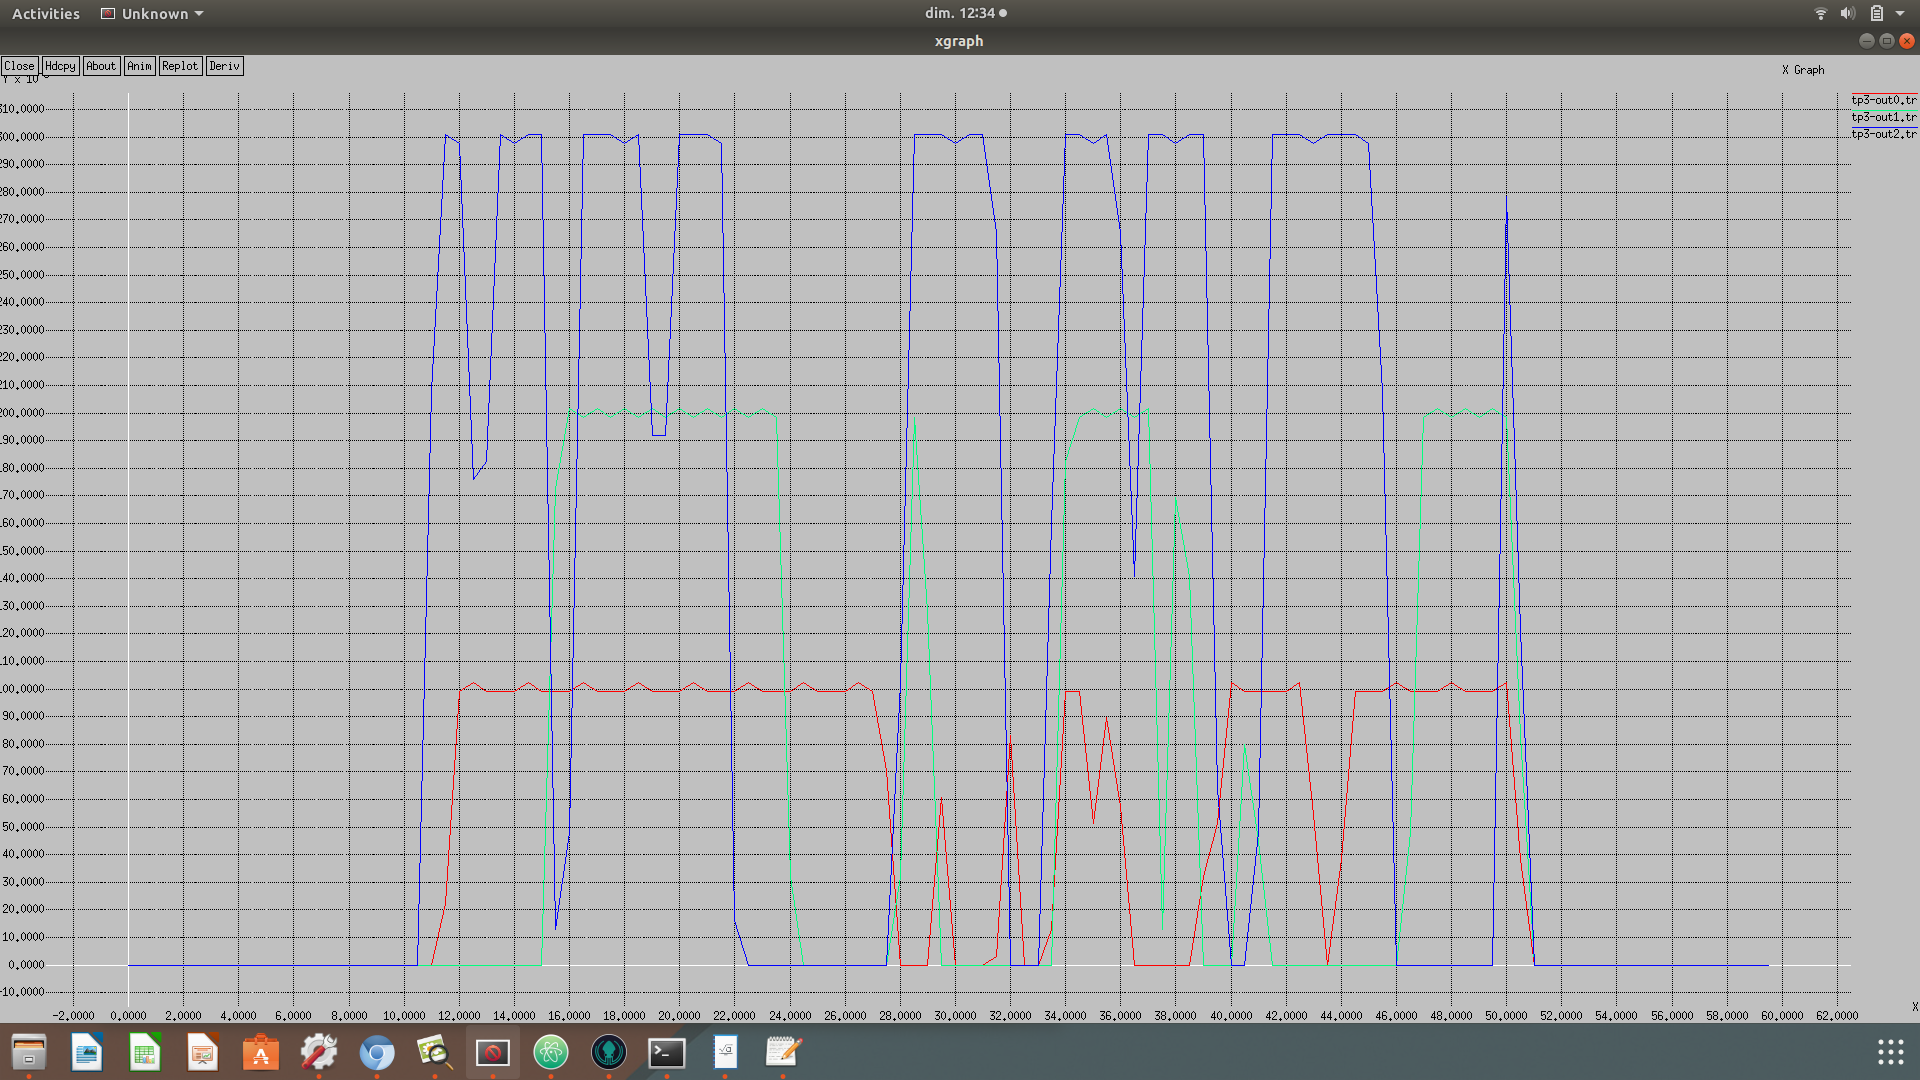
\includegraphics[width=0.99\columnwidth]{./tp3/0,5.png}
        \caption{xGraph : Échantillonage de 0.5 seconde}
    \end{figure}

    \begin{figure}
      \centering
        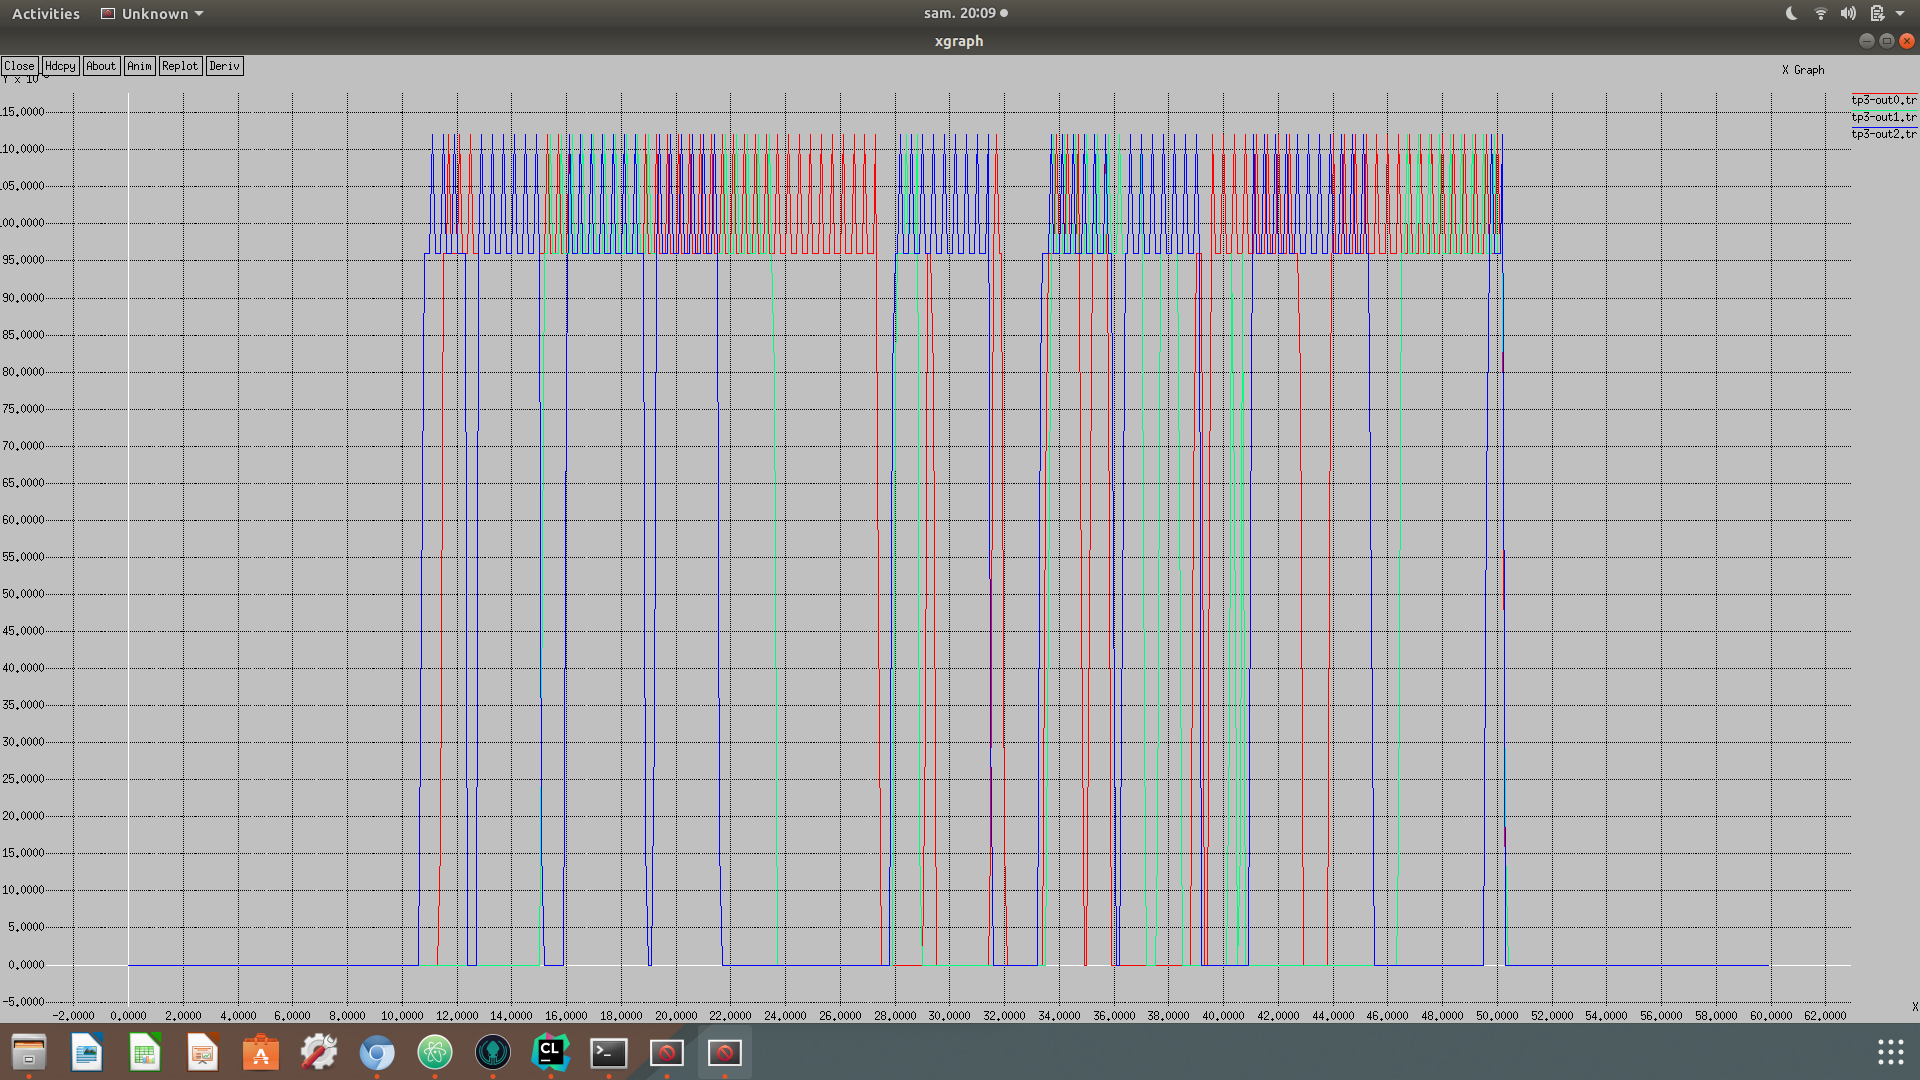
\includegraphics[width=0.99\columnwidth]{./tp3/0,1.png}
        \caption{xGraph : Échantillonage 0.1 seconde}
    \end{figure}
